Most people agrees that the dimension of a point is zero, and that of a smooth line is one, but what about a set of ordered points? One definition would be to have the dimension linked to the number of degrees of freedom needed to parametrize the object \cite{strogatz:dynamics_chaos}. A point would describe itself, and a line could be described as the curve distance from some point on the line.

This leads to the idea of fractals. Take for example the Koch curve, seen in Figure (\ref{fig:koch_curve}), it starts out as a line segment of length $L_0$, and successively adds a `bump', making the total length $L_1 = 4/3 \cdot L_0$. Iterating $n$ times gives a line length of $L_n = {(4 / 3)}^n \cdot L_0$, and so when $n$ grows to infinity, so does the length. Now each two points on the curve has at least one bump between them. However each bump has $\sim n$ bumps on it, making the length between the points infinite. This cannot be described by the curve distance between points, implying that it can not have a dimension of $1$. Although, it is not two-dimensional either since it clearly has `holes' between the lines. Consequently the dimension should be somewhere between $1$ and $2$.

A useful concept here is the similarity dimension, defined by the scaling of each iteration. If $m$ is the number of similar elements after an iteration and $r$ is the scaling factor, the dimension is defined by $m = r^d$, or equivalently

\begin{equation}
	d = \frac{\ln m}{\ln r}
\label{eq:similarityDimension}
\end{equation}

Then for the Koch curve, each segment is divided into fourths with each having one third the length from the previous iteration, giving it a dimension of $\ln 4 / \ln 3 \approx 1.26$.

\begin{figure}[h!]
    \centering
        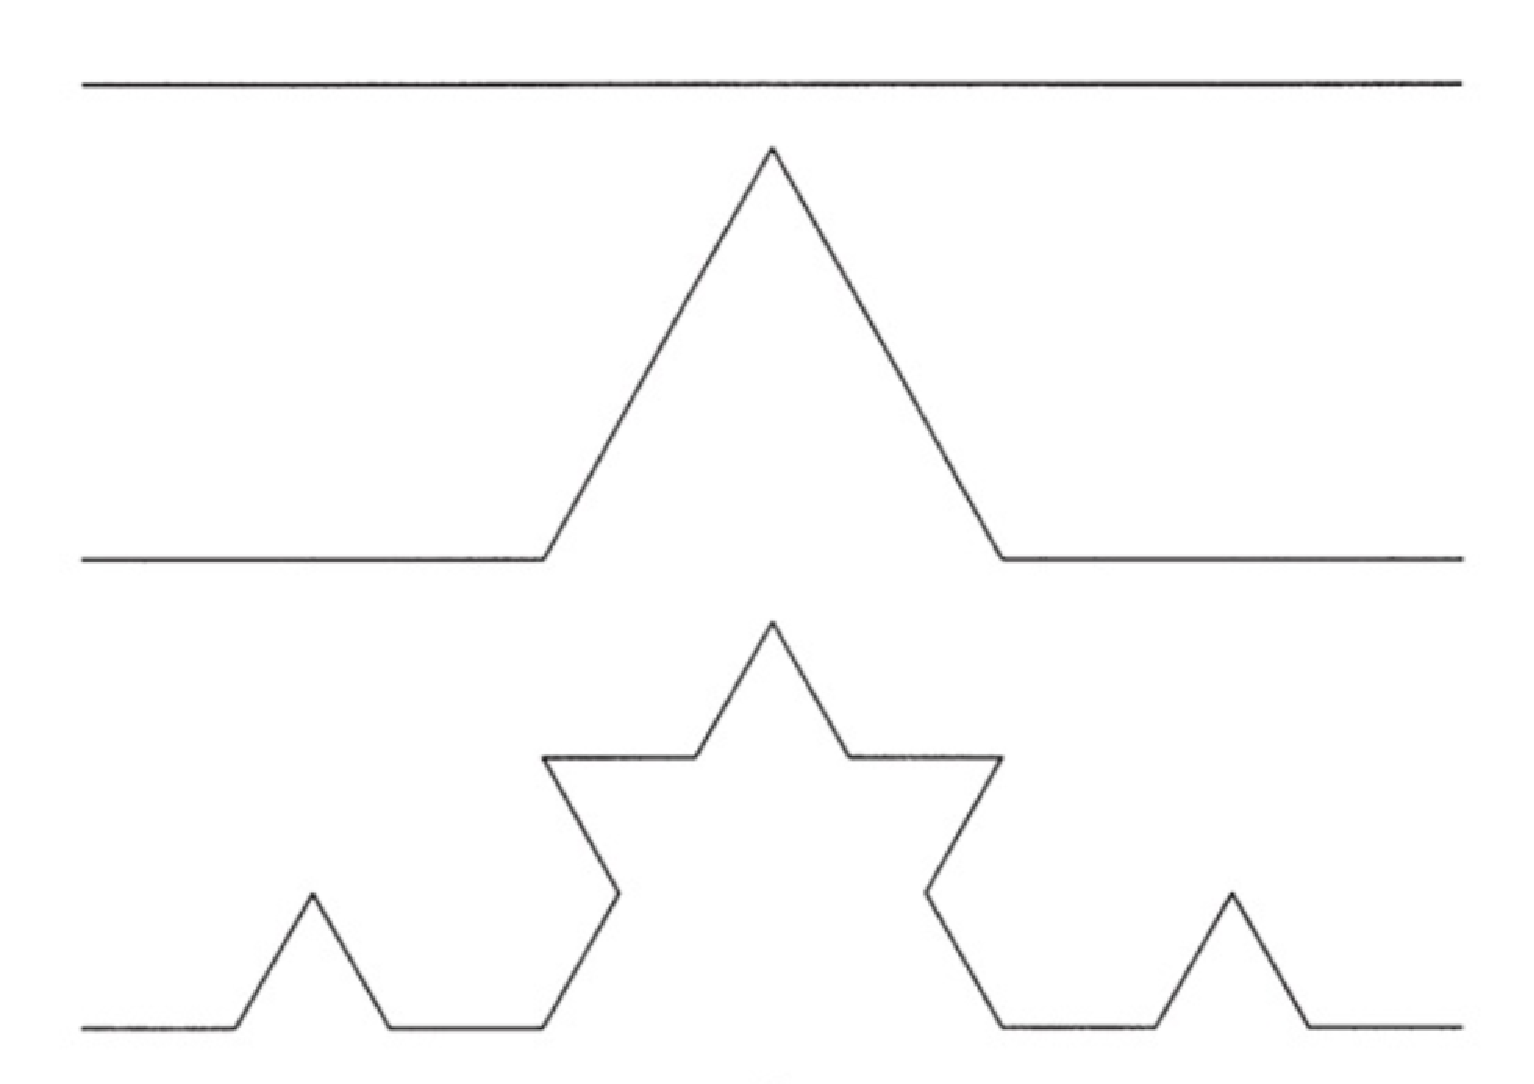
\includegraphics[width=0.8\textwidth]{figures/koch_curve.pdf}
    \caption{The Koch curve during three iterations \cite{strogatz:dynamics_chaos}.}
    \label{fig:koch_curve}
\end{figure}

The box counting method used in this thesis ressembles the method used in Equation (\ref{eq:similarityDimension}). But the scaling factor is not known, so the idea is to try to cover the fractal with a set of boxes of side length $\epsilon$. In the same way, the fractal dimension is defined as 

\begin{equation}
    d = \lim_{\epsilon \to 0} \frac{\ln N(\epsilon)}{\ln 1 / \epsilon}
\end{equation}

where $N(\epsilon)$ is the number of boxes with side length $\epsilon$ needed to cover the fractal \cite{strogatz:dynamics_chaos}.

In condensed matter physics, a lot of simulations operates on a lattice of spins, representing for example atoms in a grid. In 2001 an algorithm called the Worm algorithm was proposed \cite{Prokofev:first_worm_algorithm}. Instead of operating on individual spins, it generates spin configurations by `connecting' lattice sites together. This algorithm then generates a set of objects which have fractal like properties \cite{Duplantier:GeoHausdorff}.

The simplest such lattice is called the Ising lattice, where each spin can have one of two values. When the Worm algorithm is applied, the resulting fractal in a two dimensional Ising lattice show similar dimension to a self avoiding walk. It is proposed to be a new such type of walk where `twisted loops' are allowed where the walk is allowed to cross itself, but still has elements of self-avoidance.

The XY model adds some complexity by allowing each spin to rotate around some axis. This complexity is shown in the Worm algorithm by adding a direction and weight to the connection. Hence, instead of connecting site $a$ and site $b$, it connects site $a$ \textit{to} site $b$ with the weight $w$. There has been some contesting results of the fractal dimension of spin configurations on a $3D$ XY lattice \cite{Prokofev:comment_on_hove_hausdorff_crit_fluct}\cite{Hove:hausdorff_crit_fluctuations} and this thesis attempts to add to that discussion. 













